% docs/images/workflow.tex -- Interferosim workflow: simulation and measurement branch, common processing (TikZ, standalone)
% Version 0.1.0 (2026-11-16): first version, after the hand sketch of the workflow
% Two branches deliver the same thing -- complex baseband IQ streams of every
% station: the simulation branch (sky model -> instrument and observation ->
% IQSimulator, "Sim-Measure") and the measurement branch (antenna -> receiver
% B210 -> IQ recording, "SDR-Measure"). From the common IQ interface on, the
% chain is identical: FX correlator -> VisData -> imaging -> deconvolution.
% Dashed: shared configuration and the analytic shortcut (VisibilitySimulator).
% Used in: docs/sphinx/introduction.rst
% Build:  pdflatex workflow.tex   -> workflow.pdf
% PNG (Sphinx):  pdftoppm -r 160 -png -singlefile workflow.pdf workflow
% ================================================================
\documentclass[tikz,border=4pt]{standalone}
\usepackage{amsmath}
\usetikzlibrary{arrows.meta,positioning,calc,fit,backgrounds,shapes.geometric}

\definecolor{simbg}{RGB}{232,240,255}
\definecolor{measbg}{RGB}{226,245,226}
\definecolor{commonbg}{RGB}{255,246,214}
\definecolor{procbg}{RGB}{245,245,245}
\definecolor{nbcol}{RGB}{110,110,110}

\begin{document}
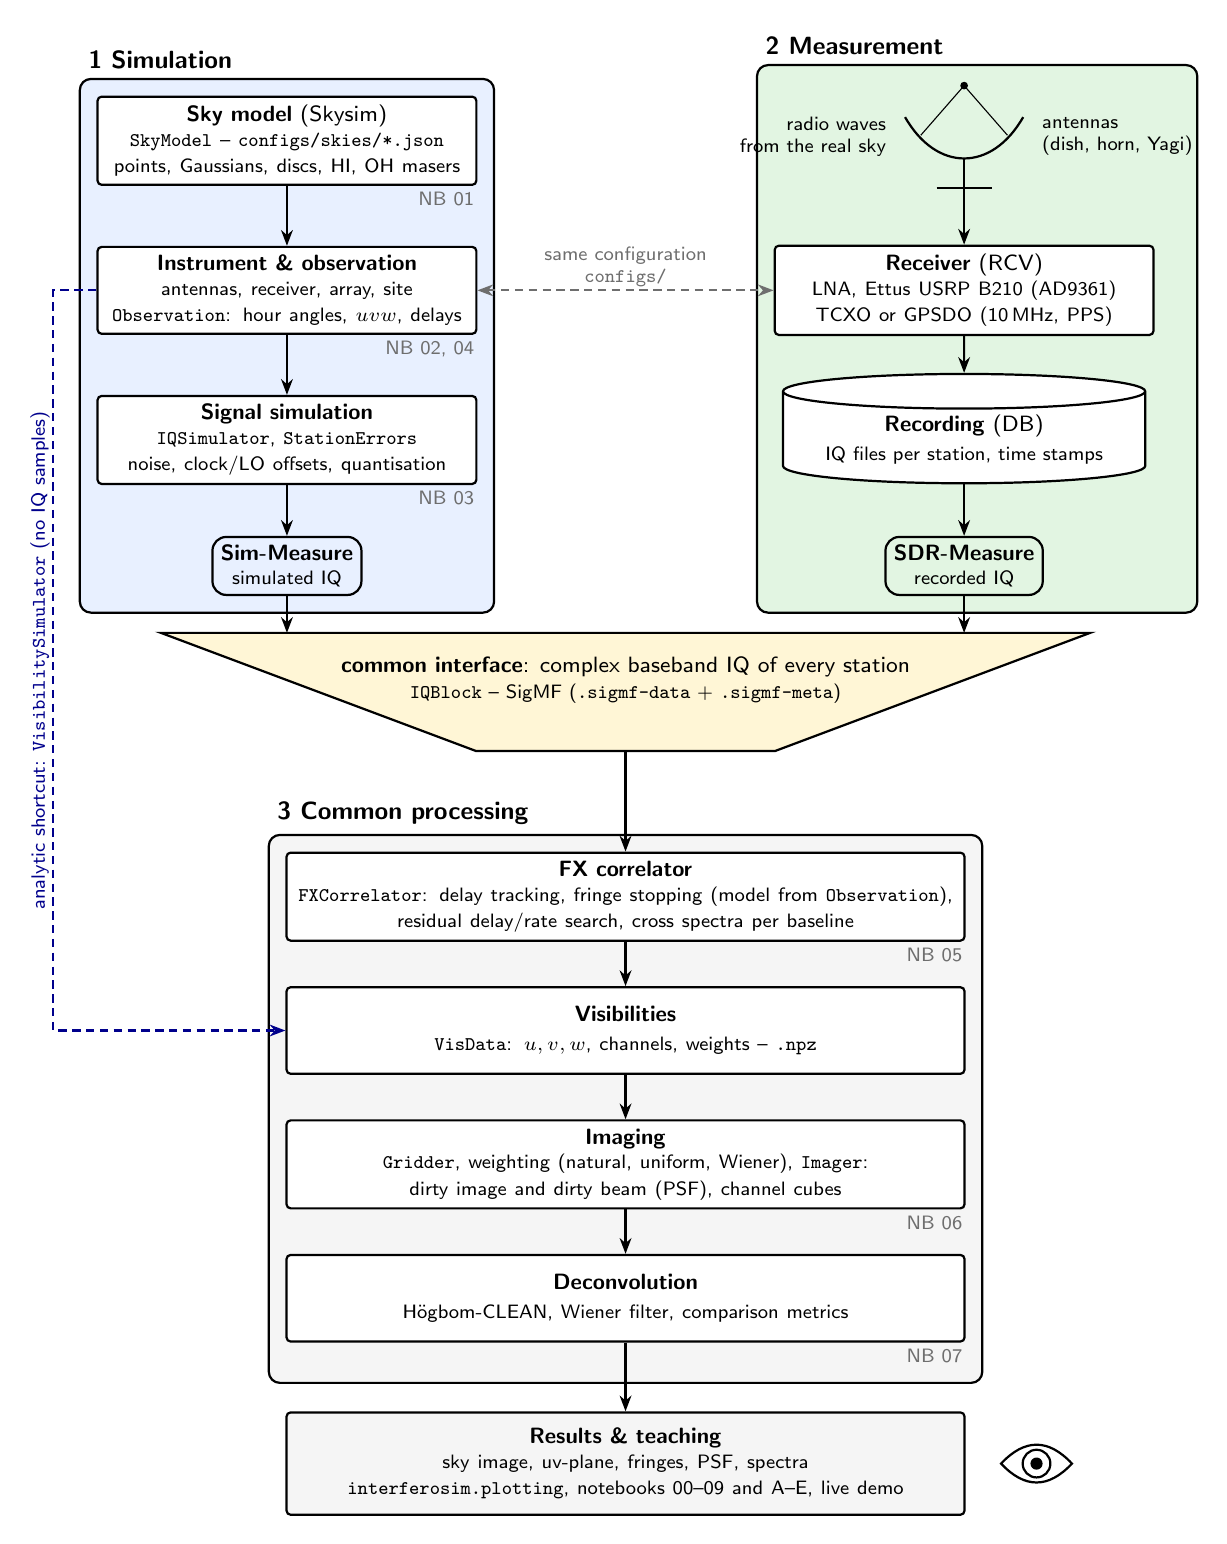
\begin{tikzpicture}[
    font=\sffamily\footnotesize,
    >={Stealth[length=2mm]},
    blk/.style={draw, thick, fill=white, rounded corners=1.5pt, align=center,
                text width=46mm, minimum height=11mm, inner sep=3pt},
    wide/.style={blk, text width=84mm},
    tag/.style={draw, thick, rounded corners=5pt, align=center, inner sep=3pt,
                font=\sffamily\footnotesize\bfseries},
    sig/.style={->, thick},
    cfg/.style={<->, thick, densely dashed, nbcol},
    byp/.style={->, thick, densely dashed, blue!55!black},
    lab/.style={font=\sffamily\scriptsize, inner sep=1pt},
    nb/.style={font=\sffamily\scriptsize, text=nbcol, inner sep=1pt, anchor=north east},
    head/.style={font=\sffamily\small\bfseries},
  ]
  \def\xl{0}      % simulation column
  \def\xr{8.6}    % measurement column
  \def\xc{4.3}    % centre

  % ------------------------------------------------------------ simulation branch
  \node[blk] (sky) at (\xl,-1.0)
    {\textbf{Sky model} (Skysim)\\[1pt]\scriptsize \texttt{SkyModel} -- \texttt{configs/skies/*.json}\\
     \scriptsize points, Gaussians, discs, HI, OH masers};
  \node[blk] (inst) at (\xl,-2.9)
    {\textbf{Instrument \& observation}\\[1pt]\scriptsize antennas, receiver, array, site\\
     \scriptsize \texttt{Observation}: hour angles, $uvw$, delays};
  \node[blk] (iqsim) at (\xl,-4.8)
    {\textbf{Signal simulation}\\[1pt]\scriptsize \texttt{IQSimulator}, \texttt{StationErrors}\\
     \scriptsize noise, clock/LO offsets, quantisation};
  \node[tag, fill=simbg] (simmeas) at (\xl,-6.4) {Sim-Measure\\[-1pt]\scriptsize\mdseries simulated IQ};
  \draw[sig] (sky) -- (inst);
  \draw[sig] (inst) -- (iqsim);
  \draw[sig] (iqsim) -- (simmeas);
  \node[nb] at ([yshift=-1pt]sky.south east)   {NB 01};
  \node[nb] at ([yshift=-1pt]inst.south east)  {NB 02, 04};
  \node[nb] at ([yshift=-1pt]iqsim.south east) {NB 03};

  % ------------------------------------------------------------ measurement branch
  % parabolic antenna with feed and mount
  \coordinate (dish) at (\xr,-1.15);
  \draw[thick] ($(dish)+(-0.75,0.45)$) .. controls ($(dish)+(-0.35,-0.25)$) and ($(dish)+(0.35,-0.25)$) .. ($(dish)+(0.75,0.45)$);
  \draw[thin] ($(dish)+(-0.55,0.22)$) -- ($(dish)+(0,0.85)$) -- ($(dish)+(0.55,0.22)$);
  \fill ($(dish)+(0,0.85)$) circle (1.4pt);
  \coordinate (dishtop) at ($(dish)+(0,0.9)$);
  \coordinate (dishright) at ($(dish)+(2.75,0)$);
  \draw[thick] ($(dish)+(0,-0.07)$) -- ($(dish)+(0,-0.45)$);
  \draw[thick] ($(dish)+(-0.35,-0.45)$) -- ($(dish)+(0.35,-0.45)$);
  \node[lab, anchor=west, align=left] at ($(dish)+(0.95,0.2)$) {antennas\\(dish, horn, Yagi)};
  \node[lab, anchor=east, align=right] at ($(dish)+(-0.95,0.2)$) {radio waves\\from the real sky};

  \node[blk] (rcv) at (\xr,-2.9)
    {\textbf{Receiver} (RCV)\\[1pt]\scriptsize LNA, Ettus USRP B210 (AD9361)\\
     \scriptsize TCXO or GPSDO (10\,MHz, PPS)};
  \node[draw, thick, fill=white, cylinder, shape border rotate=90, aspect=0.12,
        minimum height=13mm, minimum width=46mm, align=center, inner sep=2pt] (db) at (\xr,-4.8)
    {\textbf{Recording} (DB)\\[1pt]\scriptsize IQ files per station, time stamps};
  \node[tag, fill=measbg] (sdrmeas) at (\xr,-6.4) {SDR-Measure\\[-1pt]\scriptsize\mdseries recorded IQ};
  \draw[sig] ($(dish)+(0,-0.45)$) -- (rcv);
  \draw[sig] (rcv) -- (db);
  \draw[sig] (db) -- (sdrmeas);

  % shared configuration of the hardware
  \draw[cfg] (inst.east) -- node[lab, above, text=nbcol, align=center]{same configuration\\\texttt{configs/}} (rcv.west);

  % ------------------------------------------------------------ funnel: common IQ interface
  \coordinate (fTL) at (\xl-1.6,-7.25);
  \coordinate (fTR) at (\xr+1.6,-7.25);
  \coordinate (fBR) at (\xc+1.9,-8.75);
  \coordinate (fBL) at (\xc-1.9,-8.75);
  \draw[thick, fill=commonbg] (fTL) -- (fTR) -- (fBR) -- (fBL) -- cycle;
  \node[align=center] at (\xc,-7.85)
    {\textbf{common interface}: complex baseband IQ of every station\\
     \scriptsize \texttt{IQBlock} -- SigMF (\texttt{.sigmf-data} + \texttt{.sigmf-meta})};
  \draw[sig] (simmeas) -- (simmeas |- fTL);
  \draw[sig] (sdrmeas) -- (sdrmeas |- fTR);

  % ------------------------------------------------------------ common processing
  \node[wide] (corr) at (\xc,-10.6)
    {\textbf{FX correlator}\\[1pt]\scriptsize \texttt{FXCorrelator}: delay tracking, fringe stopping (model from \texttt{Observation}),\\
     \scriptsize residual delay/rate search, cross spectra per baseline};
  \node[wide] (vis) at (\xc,-12.3)
    {\textbf{Visibilities}\\[1pt]\scriptsize \texttt{VisData}: $u, v, w$, channels, weights -- \texttt{.npz}};
  \node[wide] (img) at (\xc,-14.0)
    {\textbf{Imaging}\\[1pt]\scriptsize \texttt{Gridder}, weighting (natural, uniform, Wiener), \texttt{Imager}:\\
     \scriptsize dirty image and dirty beam (PSF), channel cubes};
  \node[wide] (dec) at (\xc,-15.7)
    {\textbf{Deconvolution}\\[1pt]\scriptsize Högbom-CLEAN, Wiener filter, comparison metrics};
  \draw[sig] ($(fBL)!0.5!(fBR)$) -- (corr);
  \draw[sig] (corr) -- (vis);
  \draw[sig] (vis) -- (img);
  \draw[sig] (img) -- (dec);
  \node[nb] at ([yshift=-1pt]corr.south east) {NB 05};
  \node[nb] at ([yshift=-1pt]img.south east)  {NB 06};
  \node[nb] at ([yshift=-1pt]dec.south east)  {NB 07};
  \coordinate (decnb) at ($(dec.south)+(0,-0.3)$);

  % analytic shortcut without IQ samples
  \draw[byp] (inst.west) -- ++(-0.55,0) coordinate (b1) -- (b1 |- vis.west) -- (vis.west);
  \node[lab, text=blue!55!black, rotate=90, anchor=south] at ($(b1)!0.5!(b1 |- vis.west)$)
    {analytic shortcut: \texttt{VisibilitySimulator} (no IQ samples)};

  % ------------------------------------------------------------ results
  \node[blk, text width=84mm, minimum height=13mm, fill=procbg] (res) at (\xc,-17.8)
    {\textbf{Results \& teaching}\\[1pt]\scriptsize sky image, uv-plane, fringes, PSF, spectra\\
     \scriptsize \texttt{interferosim.plotting}, notebooks 00--09 and A--E, live demo};
  \draw[sig] (dec) -- (res);
  % eye: the user looks at the result
  \coordinate (eye) at ($(res.east)+(0.9,0)$);
  \draw[thick] ($(eye)+(-0.45,0)$) .. controls ($(eye)+(-0.15,0.32)$) and ($(eye)+(0.15,0.32)$) .. ($(eye)+(0.45,0)$)
               .. controls ($(eye)+(0.15,-0.32)$) and ($(eye)+(-0.15,-0.32)$) .. cycle;
  \fill ($(eye)$) circle (2.2pt);
  \draw[thick] (eye) circle (5pt);

  % ------------------------------------------------------------ frames and headings
  \begin{scope}[on background layer]
    \node[draw, thick, fill=simbg, rounded corners=4pt, inner sep=6pt,
          fit=(sky)(inst)(iqsim)(simmeas)] (simframe) {};
    \node[draw, thick, fill=measbg, rounded corners=4pt, inner sep=6pt,
          fit=(rcv)(db)(sdrmeas)(dishtop)(dishright)] (measframe) {};
    \node[draw, thick, fill=procbg, rounded corners=4pt, inner sep=6pt,
          fit=(corr)(vis)(img)(dec)(decnb)] (procframe) {};
  \end{scope}
  \node[head, anchor=south west] at (simframe.north west)  {1\,\,Simulation};
  \node[head, anchor=south west] at (measframe.north west) {2\,\,Measurement};
  \node[head, anchor=south west] at (procframe.north west) {3\,\,Common processing};
\end{tikzpicture}
\end{document}
